\documentclass[twoside]{article}

\usepackage{fancyhdr}
\usepackage{geometry}
\usepackage{chemfig}
\usepackage{amsmath}
\usepackage{pgfplots}
\usepackage{rotating}
\usepackage{multicol}
\usepackage{tikz}
\usetikzlibrary{arrows,positioning,shapes.geometric}
\usepgfplotslibrary{polar}

\geometry{
    top=20mm,
    bottom=30mm,
    left=20mm,
    right=20mm
}

\pagestyle{fancy}
\renewcommand{\headrulewidth}{0pt}
\fancyfoot[LO]{
    \begin{turn}{180}
        \begin{minipage}{0.4\linewidth}
            \begin{flushright}
                \begin{multicols}{2}
                    \emph{written exclusively under the influence}
                    \begin{turn}{90}
                    \chemfig{[,0.4]*6(([,0.5]=)-([6,0.7]-)-*5(-=-([:60, 0.7]-)-=)--([,0.5]=)-([:150, 0.7]-)-)}
                    \end{turn}
                \end{multicols}
            \end{flushright}
        \end{minipage}
    \end{turn}
}


\title{\underline{A treatise on non-aquatic gastropod Mollusca, a.k.a. \emph{snails}}}
\author{Aayush Bajaj}
\date{\today}

\begin{document}

\maketitle % this command implicitly changes the pagestyle to 'title' (duh!)
\thispagestyle{fancy}

\dotfill
\bigbreak

\section*{Definitions}

    \begin{flushright}
    \begin{minipage}{8cm}
        \begin{flushleft} \emph{If you wish to converse with me define your terms.} \end{flushleft}
        \begin{flushright}--- Voltaire\end{flushright}
    \end{minipage}
    \end{flushright}

    Snails are defined as gastropods that have a shell. Gastropods are a \underline{class} of invertebrates which include slugs, squids, octupuses \emph{and} snails. These gastropods belong to a \textbf{larger} \underline{phylum} of animals called \emph{Mollusca}.

\section*{Classifications}
    The gastropod class includes both aquatic and non-aquatic snails and are the most diverse class of \emph{Molluscs}, residing in \textbf{every} marine environment from high-energy surge zones to ocean floorbeds.

    Restricting our study to \emph{non-aquatic} gastropods brings us to 2 particular \underline{families}; the \textbf{prosobranchia} and the \textbf{pulmonata}.

    \subsection*{Prosobranchia}
        
    \subsection*{Pulmonata}


    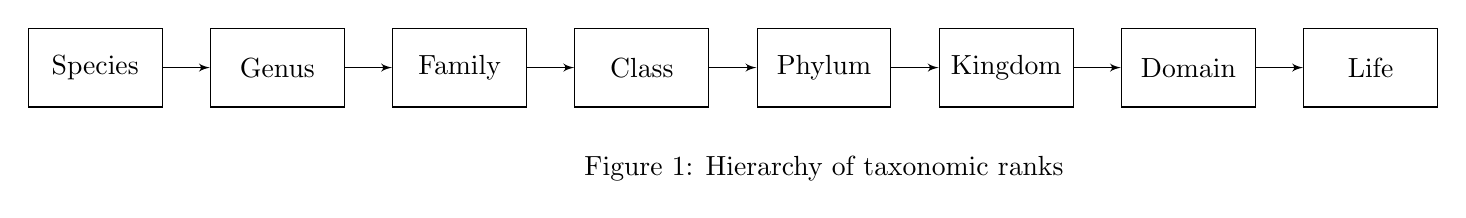
\begin{tikzpicture}[>=latex']
    \centering
        \tikzset{block/.style= {draw, rectangle, align=center,minimum width=1.7cm,minimum height=1cm}}
        \node [block] (species) {Species};
        \node [block, right =0.6cm of species] (genus) {Genus};
        \node [block, right =0.6cm of genus] (family) {Family};
        \node [block, right =0.6cm of family] (class) {Class};
        \node [block, right =0.6cm of class] (phylum) {Phylum};
        \node [block, right =0.6cm of phylum] (kingdom) {Kingdom};
        \node [block, right =0.6cm of kingdom] (domain) {Domain};
        \node [block, right =0.6cm of domain] (life) {Life};

        \path[draw,->] (species) edge (genus)
                    (genus) edge (family)
                    (family) edge (class)
                    (class) edge (phylum)
                    (phylum) edge (kingdom)
                    (kingdom) edge (domain)
                    (domain) edge (life)
                    ;
        \node [below=1cm, align=flush center,text width=8cm] at (phylum) { Figure 1: Hierarchy of taxonomic ranks };
    \end{tikzpicture}

\section*{Habitat}
    
\section*{Behaviours}

\newpage

\begin{multicols}{2}

    \begin{minipage}{0.4\textwidth}
    \section*{Facts}
        Snails are hermaphrodites, they all have pp
    \end{minipage}

    \begin{flushleft}
    \begin{minipage}{0.5\textwidth}
    \section*{Mathematics}

        Let us briefly consider the length of Jamiroquai the Garden Snail \emph{(a.k.a cornu aspersum)}.
        Approximating the shell function to be defined in polar coordinates as \(r = e^{\frac{-\theta}{10}}\) we may then use \[ l = \int^{\theta_1}_{\theta_0} \sqrt{[f(\theta)]^2 + [f'(\theta)]^2} \, \mathrm{d}\theta .\]

        On

        \begin{center}
            \begin{tikzpicture}
                \node[inner sep=0pt] (snail) at (0,0)
                    {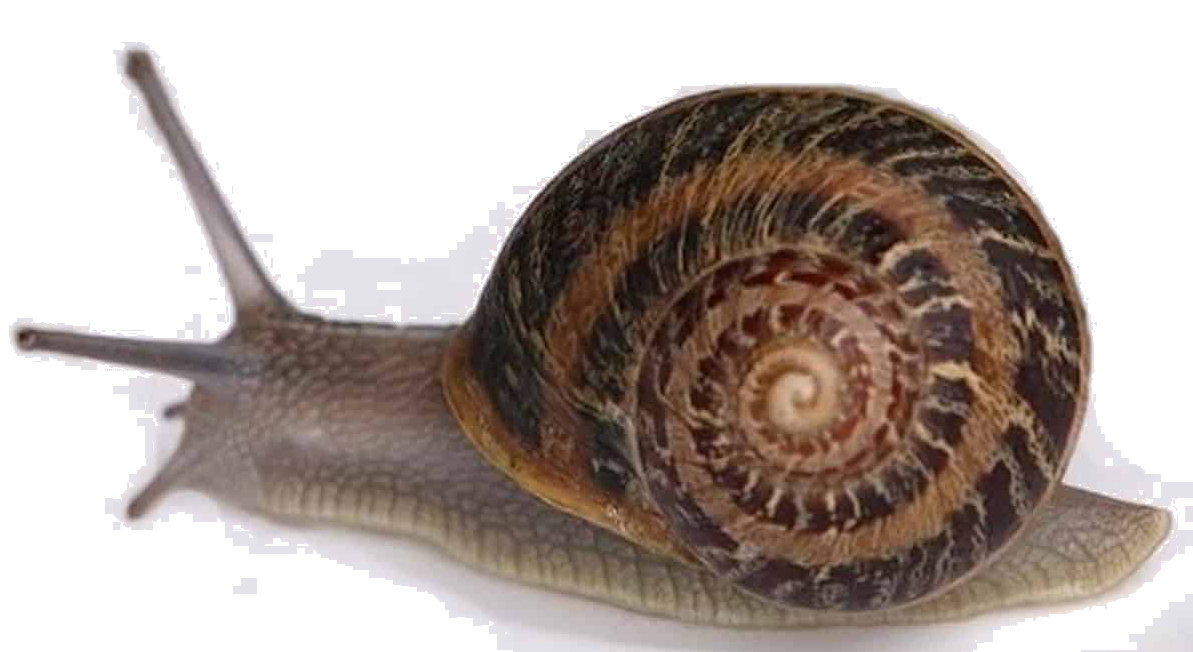
\includegraphics[width=.5\textwidth]{img/snail.png}};
                \node[inner sep=0pt] (spiral) at (-1.3,-1.6) {
                    \begin{polaraxis}[axis lines=none, scale = .4]
                        \addplot[domain=0:1260, samples=1000, line width = 1mm]{e^0.1*x};
                    \end{polaraxis}
                    };
                    \node [below=1cm, align=flush center,text width=8cm] at (spiral) { Figure 2: Jamiroquai };
            \end{tikzpicture}
        \end{center}

        Such that the unravelled length of Mr Aspersum's shell becomes 
        \begin{align*}
            l &= \int^{\theta_1}_{0} \sqrt{(e^{-\frac{\theta}{10}})^2 + (-\frac{1}{10}e^{-\frac{\theta}{10}})^2}\mathrm{d}\theta\\
            &= \int^{\theta_1}_{0} \sqrt{(1+\frac{1}{100})e^{-\frac{2\theta}{10}}} \mathrm{d}\theta\\
            &= \frac{\sqrt{101}}{10} \int^{\theta_1}_0 e^{-\frac{\theta}{10}}\mathrm{d}\theta\\
            &= \sqrt{101}(1 - e^{-\frac{\theta_1}{10}}).\\
            &= \sqrt{101} \text{ (as \(\theta_1 \rightarrow \infty\)).}
        \end{align*}

    \end{minipage}
    \end{flushleft}

\end{multicols}

\section*{Glossary}
Phylum
Herbivore, Omnivore, Carnivore
\section*{References}



Snails are defined as gastropods that have a shell. 

This shall be a fun exercise. I will need to learn how to produce a tree diagram in \LaTeX{} as well as a TikZ picture of a golden spiral overlaid atop a snail (at the very least).

To accomplish the latter I shall leverage the arc length of a curve as \(\theta_1 \rightarrow \infty\) for \(l\), where


Then for a given curve such as \(r = e^\frac{\theta}{10}\):

The length of the arc is:

\end{document}
